\documentclass[12pt,letterpaper]{article}


\usepackage[top=1in, 
		    bottom=1in,
		    left=1in,
		    right=1in]{geometry}
\usepackage{setspace}	% makes the \singlespacing, \onehalfspacing, and \doublespacing commands available
% \usepackage[en-US]{datetime2}
% \DTMlangsetup{showdayofmonth=false}
% \usepackage{titlesec}
\usepackage{listings}	% allows for placing programming code to be displayed correctly
\usepackage{siunitx}	% units
\usepackage{amsmath}
\usepackage{amsfonts}
\usepackage{amssymb}
\usepackage{graphicx}
\usepackage{booktabs}
\usepackage{multirow}
\usepackage{pgfplots}
\pgfplotsset{compat=newest}
\usepackage{tikz}
%\usetikzlibrary{shapes.geometric}
% \usepgfplotslibrary{external} 
% \tikzexternalize[prefix=pdfimages/,
% 		        mode=list and make]
\usepackage{caption}
\usepackage[list=true,
		     listformat=simple]{subcaption}
%\usepackage{cleveref}	% this should really go last
% \usepackage[colorlinks,
% 		     linkcolor=black,
% 		     citecolor=black,
% 		     plainpages=false,
% 		     pdfpagelabels]{hyperref}
% \usepackage[all]{hypcap}
\usepackage{cleveref}
% \doublespacing

\pagenumbering{gobble}
\newcommand{\mymder}[2]{\ensuremath{\frac{\mathrm{D}#1}{\mathrm{D}#2}}}
\newcommand{\mypder}[2]{\ensuremath{\frac{\partial #1}{\partial #2}}}
\newcommand{\mypdertwo}[2]{\ensuremath{\frac{\partial^2 #1}{\partial #2^2}}}
\newcommand{\mymdervec}[1]{\ensuremath{mypder{#1}{t} + }}
\newcommand{\myder}[2]{\ensuremath{\frac{d#1}{d#2}}}
\newcommand{\mydiv}[1]{\ensuremath{\nabla \cdot {#1}}}
\newcommand{\myfrac}[2]{\ensuremath{^{#1}\!/_{#2}}}
\newcommand{\myfunc}[2]{\ensuremath{#1 \left( #2 \right)}}
\newcommand{\myparen}[1]{\ensuremath{\left( #1 \right)}}
\newcommand{\mybrack}[1]{\ensuremath{\left[ #1 \right]}}
\newcommand{\mybrace}[1]{\ensuremath{\left\{ #1 \right\}}}
\newcommand{\mysin}[1]{\ensuremath{\myfunc{\mathrm{sin}}{#1}}}
\newcommand{\mycos}[1]{\ensuremath{\myfunc{\mathrm{cos}}{#1}}}
\newcommand{\myexp}[1]{\ensuremath{\myfunc{\mathrm{exp}}{#1}}}
\newcommand{\myint}[4]{\ensuremath{\int_{#1}^{#2} {#3} d {#4}}}


\newcommand{\Rld}{\ensuremath{\mathit{Re}}}
\newcommand{\St}{\ensuremath{\mathit{St}}}
\newcommand{\Prn}{\ensuremath{\mathit{Pr}}}
\newcommand{\Sc}{\ensuremath{\mathit{Sc}}}
\newcommand{\Sh}{\ensuremath{\mathit{Sh}}}
\newcommand{\Nu}{\ensuremath{\mathit{Nu}}}
\newcommand{\Bi}{\ensuremath{\mathit{Bi}}}


\let\textacute\'
\let\textgrave\`


\newcommand{\includetikz}[2]{%
    \tikzsetnextfilename{#2}%
    \input{#1#2.tex}%
}

\begin{document}

\noindent
MECH 131A Homework 1

\noindent
Assigned date: October $1^{\mathrm{st}}$, 2024

\noindent
Due date: October $11^{\mathrm{th}}$, 2024

\subsubsection*{Problem Set}
\begin{enumerate}

\item  (Problem 3.11 in FHMT) A house has a composite wall of wood, fiberglass insulation, and plaster board (as indicated in the sketch below).
On a cold winter day, the convection heat transfer coefficients are $h_o = \SI{60}{\watt\per\square\meter\per\kelvin}$ and $h_i = \SI{30}{\watt\per\square\meter\per\kelvin}$.
The total wall surface area is \SI{350}{\square\meter}.

\begin{figure}[!htpb]
	\centering
	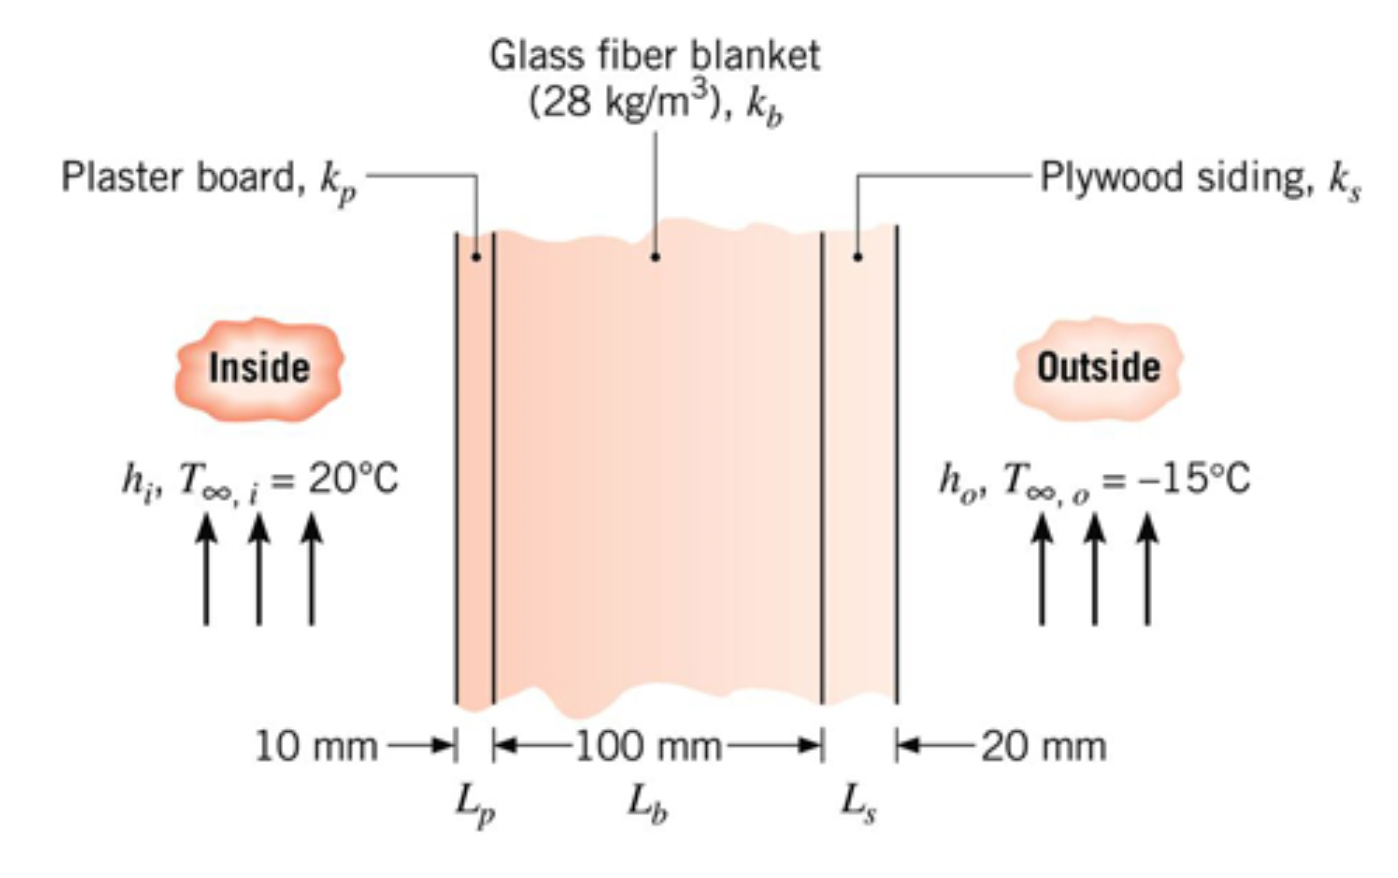
\includegraphics[width=0.75\linewidth]{./image0.png}
\end{figure}

	\begin{enumerate}
		\item Determine a symbolic expression for the total thermal resistance of the wall, including inside and outside convection effects for the prescribed conditions.
		\item Determine the total rate of heat loss through the wall.
		\item If the wind were blowing violently, raising $h_o$ to $\SI{300}{\watt\per\square\meter\per\kelvin}$, determine the percentage increase in the rate of heat loss.
		\item What is the controlling resistance that determines the amount of the heat flow through the wall?
	\end{enumerate}

\item (Problem 3.14 in FHMT) Consider a composite wall that includes an \SI{8}{\milli\meter} thick hardwood siding, \SI{40}{\milli\meter} by \SI{130}{\milli\meter} hardwood studs on \SI{0.65}{\meter} centers with glass fiber insulation (paper faced, \SI{28}{\kilogram\per\cubic\meter}), and a \SI{12}{\milli\meter} layer of gypsum (vermiculite) wall board.

\begin{figure}[!htpb]
	\centering
	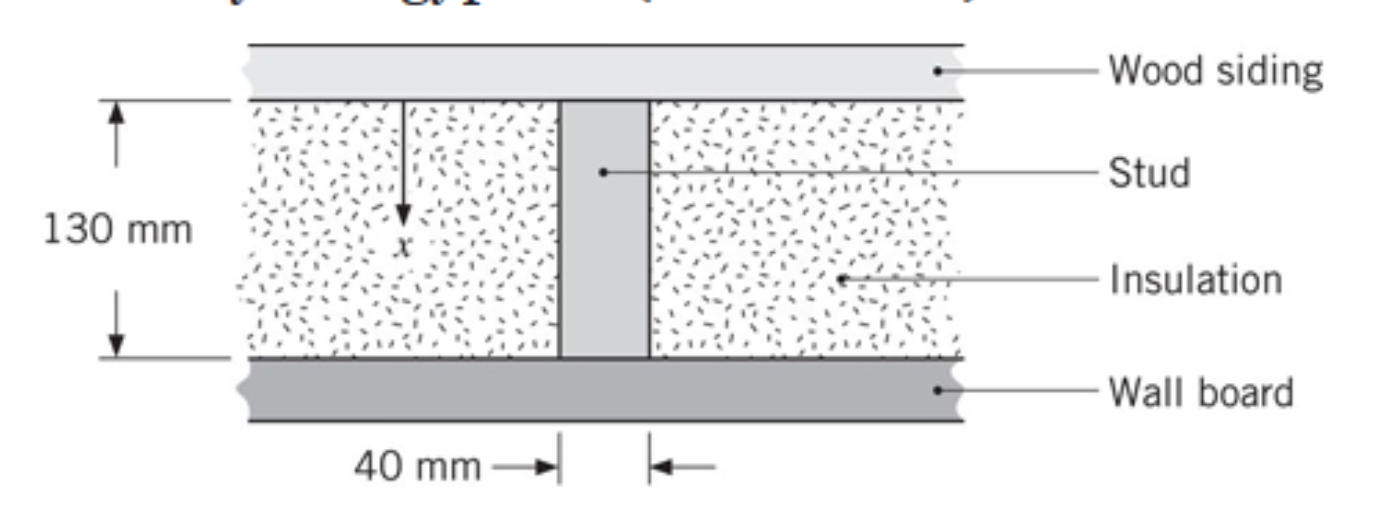
\includegraphics[width=0.75\linewidth]{./image1.png}
\end{figure}

\noindent
What is the thermal resistance associated with a wall that is \SI{2.5}{\meter} high by \SI{6.5}{\meter} wide (having 10 studs, each \SI{2.5}{\meter} high)?
Assume surfaces normal to the $x$-direction are isothermal.

%\item A composite cylindrical wall is composed of two materials of thermal conductivity of $k_A$ and $k_B$, which are separated by a very thin, electric resistance heater for which interfacial contact resistance is negligible (see image above).
%\begin{figure}[!htpb]
%	\centering
%	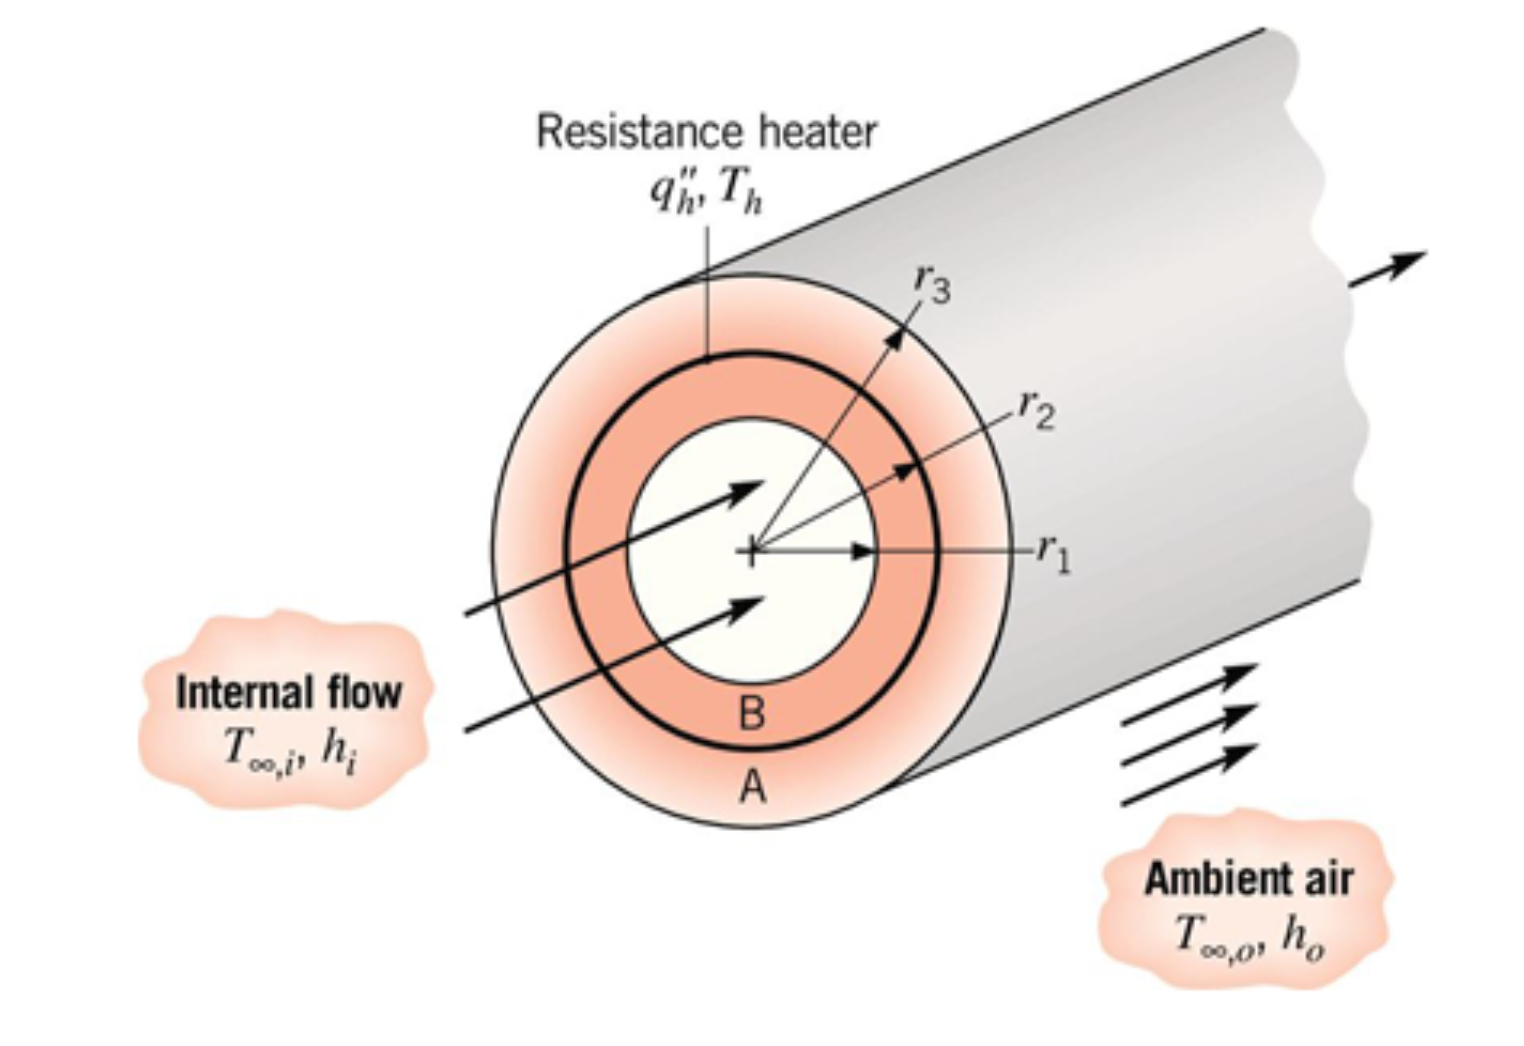
\includegraphics[width=0.75\linewidth]{./image2.png}
%\end{figure}
%
%\noindent
%Liquid pumped through the tube is at a temperature $T_{\infty, i}$ and provides a convection coefficient $h_i$ at the inner surface of the composite.
%The outer surface is exposed to the ambient air, which is at $T_{\infty,o}$, and provides a convection coefficient of $h_o$.
%Under steady-state conditions, a uniform heat flux of $q''_h$ is dissipated by the heater.
%
%	\begin{enumerate}
%		\item Sketch the equivalent thermal circuit of the system and express all resistance in terms of relevant variables.
%		\item Obtain an expression that may be used to determine the heater temperature $T_h$.
%		\item Obtain an expression for the ratio of the heat flow to the outer and inner fluids, $q_0' /  q_i'$.
%		How might the variables of the problem be adjusted to minimize this ratio?
%		\item Redo (a)-(c) if there is boiling on the inner surface instead of convection.
%		Compare the results.
%	\end{enumerate}

%\item It is proposed to air-cool the cylinders of a combustion chamber by joining an aluminum casing with annular fins ($k = \SI{240}{\watt\per\meter\per\kelvin}$) to the cylinder wall ($k = \SI{50}{\watt\per\meter\per\kelvin}$).
%
%\begin{figure}[!htpb]
%	\centering
%	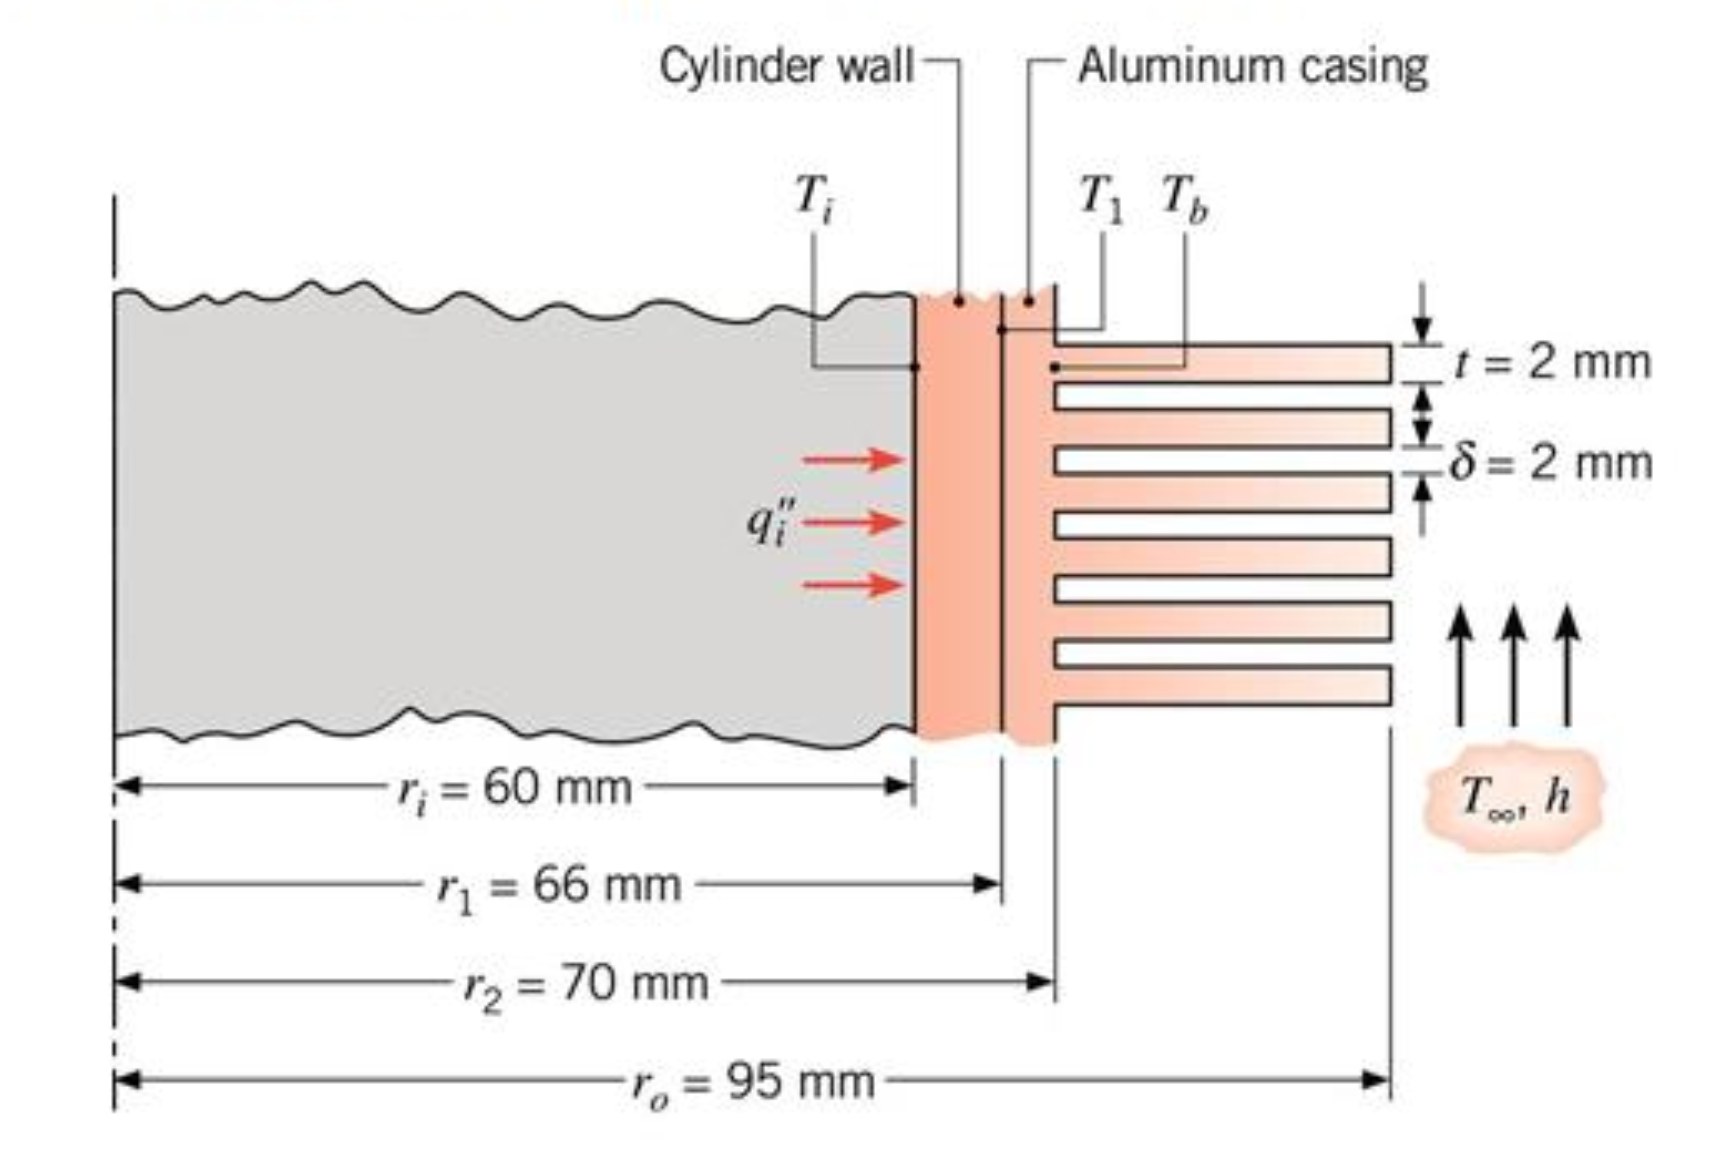
\includegraphics[width=0.75\linewidth]{./image3.png}
%\end{figure}
%
%The air is at \SI{320}{\kelvin} and the corresponding convection coefficient is \SI{100}{\watt\per\square\meter\per\kelvin}.
%Although heating at the inner suface is periodic, it is reasonable to assume steady-state conditions with a time-averaged heat flux of $q''_i = \num{1d5} \si{\watt\per\square\meter}$.
%Assuming negligible contact resistance between the wall and the casing, determine the wall inner temperature $T_i$, the interface temperature $T_1$, and the fin base temperature $T_b$.
%Determine these temperatures if the interface contact resistance is $R_{t,c}'' = \num{1d-4} \si{\square\meter\kelvin\per\watt}$.


\item Recreate the plot below using MATLAB or Python without the adiabatic tip simplification, i.e. use $L$ not $L_c$.

\begin{figure}[!htpb]
	\centering
	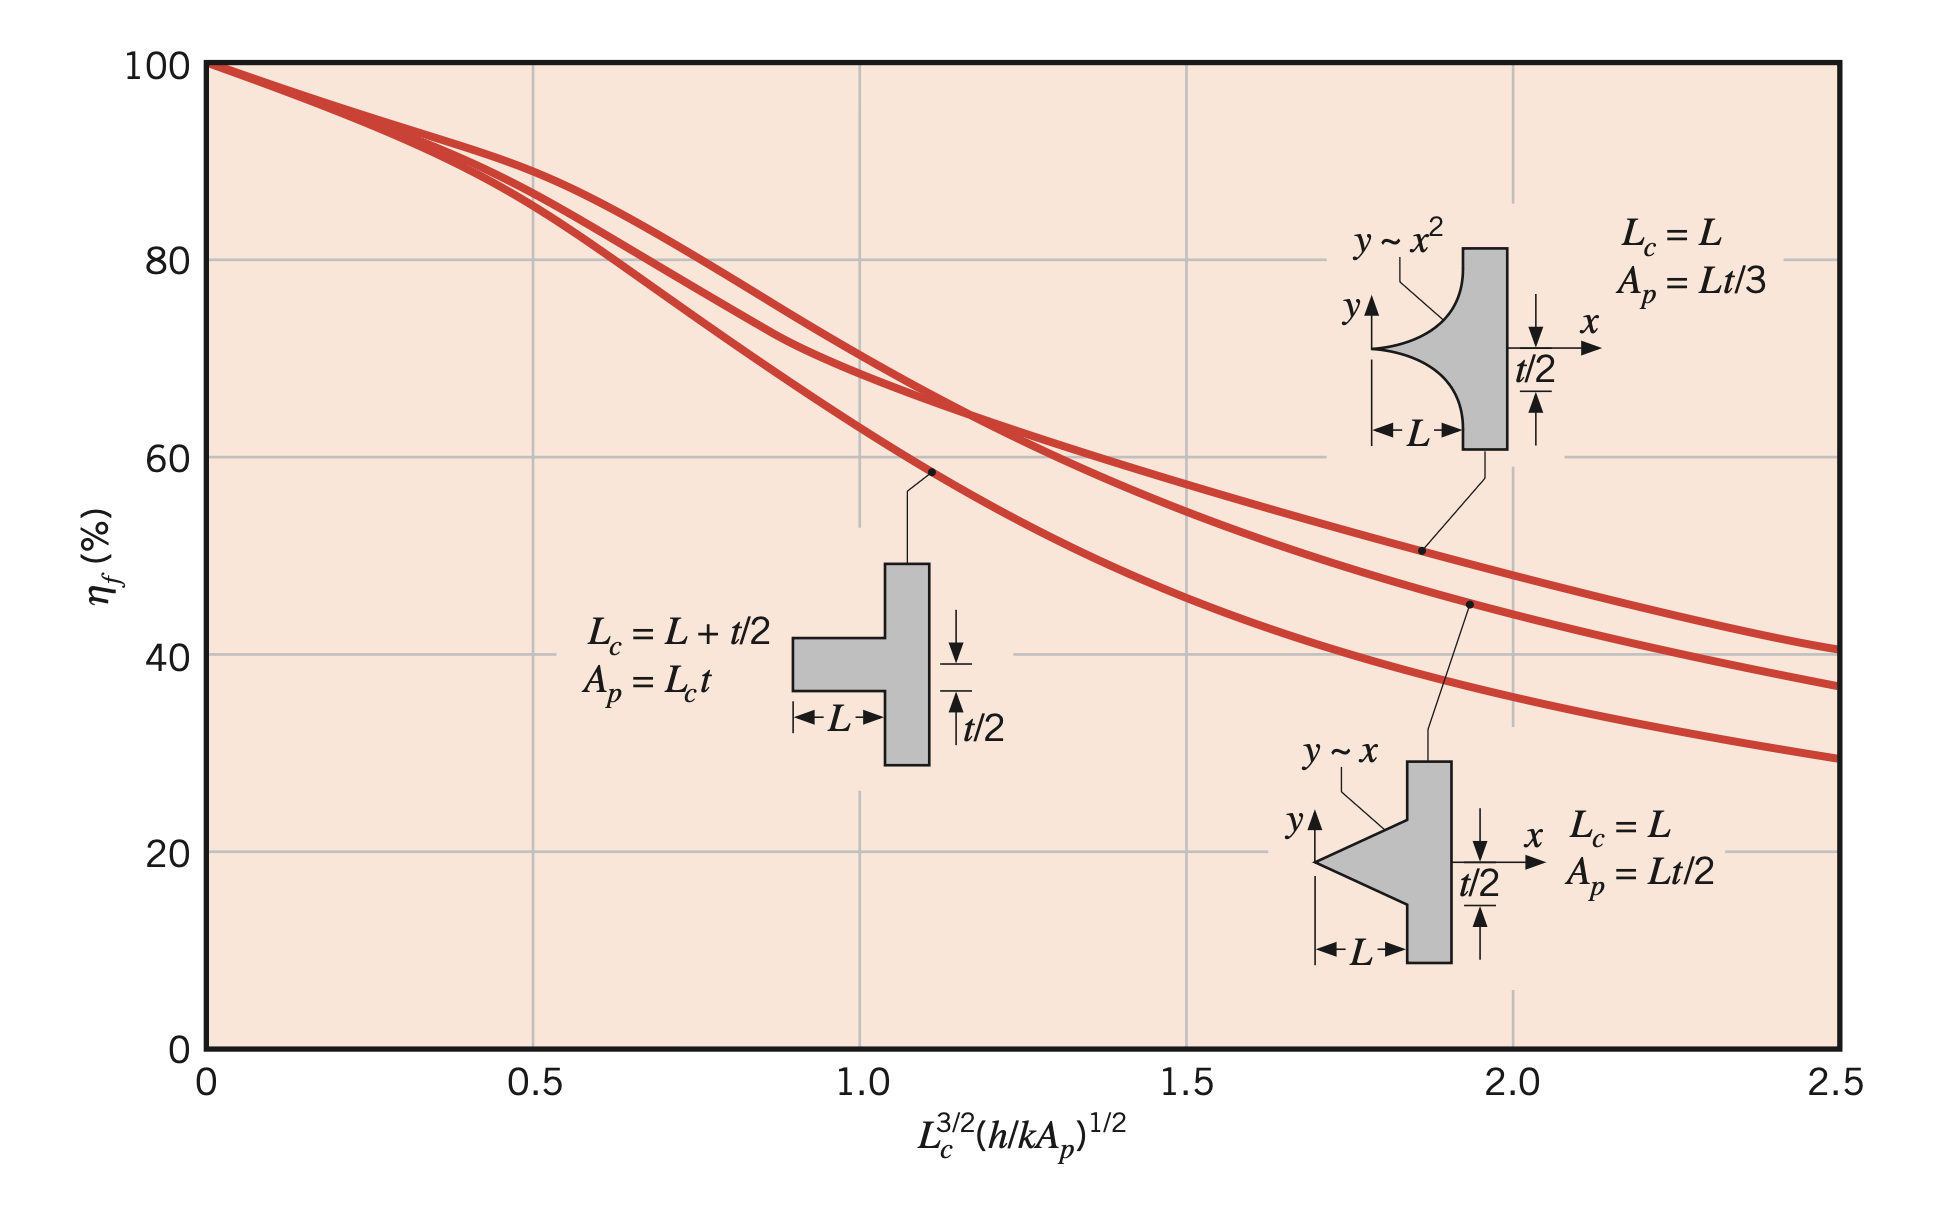
\includegraphics[width=0.75\linewidth]{./image4.png}
\end{figure}

	\begin{enumerate}
		\item Write the second order ODE describing the fin equation as a system of equations with a change of variables $T = y_0$ and $\mypder{T}{x} = y_1$.
		Keep the change in area terms.
		\item Solve the fin equation for the ``infinite fin'' set of boundary conditions with a constant cross sectional area using an ode solver in either MATLAB or Python and compare to the analytical solution.
		How long does the fin need to be before the solutions compare well?
		\item Now we're going to solve the fin equation for a rectangular fin with a convective tip.
		Wrap the ode solver in an minimization function to solve for the missing initial value required to integrate the system of ODEs as an initial value problem.
		The error minimized should be the square of the difference between the desired tip condition and the tip condition at the tip from the numerical integration.
		You can assume the heat transfer coefficient at the tip is the same along the fin.
		You will likely have to assume values of the base temperature, thermal conductivity, heat transfer coefficient, cross sectional area, wetted perimeter, and fin length.
		\item Verify the heat flux at the base of the fin supplied by the solution to (c) is the same as the total convective heat losses along the length of the fin.
		Why should they match?
		\item Now that you can numerically solve the fin equation for an arbitrary fin, vary $m L$ and recreate the graph above for the three shapes shown.
		Don't forget to include the area variation along the length of the fin!
		Describe why assuming base temperature, thermal conductivity, heat transfer coefficient, cross sectional area, wetted perimeter, and fin length do not invalidate the process of recreating the graph.
		\item Do your results agree with the plot?
		If not, why?
	\end{enumerate}

\end{enumerate}


\end{document}